\documentclass[11pt, oneside]{article}   	% use "amsart" instead of "article" for AMSLaTeX format
\usepackage{geometry}                		% See geometry.pdf to learn the layout options. There are lots.
\geometry{letterpaper}                   		% ... or a4paper or a5paper or ... 
%\geometry{landscape}                		% Activate for for rotated page geometry
%\usepackage[parfill]{parskip}    		% Activate to begin paragraphs with an empty line rather than an indent
\usepackage{graphicx}				% Use pdf, png, jpg, or eps� with pdflatex; use eps in DVI mode
								% TeX will automatically convert eps --> pdf in pdflatex		
\usepackage{amssymb}
\usepackage{fancyref,multicol,fixltx2e,gensymb}
\usepackage{setspace}
\onehalfspacing

\title{A Microfluidic Device for Measuring Aerotaxis}
\author{Kiarash Adl, Brian Djaja, Katarina Struckmann and Logan Williams}
%\date{}							% Activate to display a given date or no date

\begin{document}
\maketitle
\tableofcontents
\newpage

\section{Abstract}

Bacteria rely heavily on sensing environmental gradients to survive and reproduce. While significant effort has been made to understand responses to chemical gradients, or chemotactic responses, less literature exists characterizing responses to gas gradients, or aerotactic responses. This study employed a three-channel microfluidic device fabricated from PDMS to characterize aerotactic bacterial motion. In the presence of a gradient of nitrogen and oxygen, movement of the organism \textit{B. subtilis} tended toward oxygen and away from nitrogen, demonstrating an aerotactic response.

\section{Introduction}

The movement of bacteria in response to a gas gradient, aerotaxis, is a field that has emerged within the past 15 years \cite{15years}. As such, it has not been studied to the extent of the similar process chemotaxis. Chemotaxis is the movement of bacteria in response to a chemical gradient, where the chemical can be anything from food to toxic molecules. Models for chemotaxis in bacteria have been characterized both for populations and single bacterial cells \cite{modelI} \cite{modelII}.

Aerotaxis was studied in a microfluidic device using a custom optical microscope. The microfluidic device allowed for development of a gas gradient along its length; the bacteria�s response to the gradient was visualized with the microscope. This setup can be utilized for studying different bacteria species and potentially other cell types. 

Aerotaxis has a broad range of applications; the signaling proteins utilized in for aerotactic responses in bacteria can be engineered for turning on gene expression in the presence of a certain oxygen concentration, or lack thereof. Since aerotaxis occurs on the order of minutes, a response can be expressed fairly rapidly. Additionally, modeling aerotaxis is key to understanding how applications such as the aforementioned can be utilized.

\section{Experimental apparatus}
\begin{figure} 
	\centering
    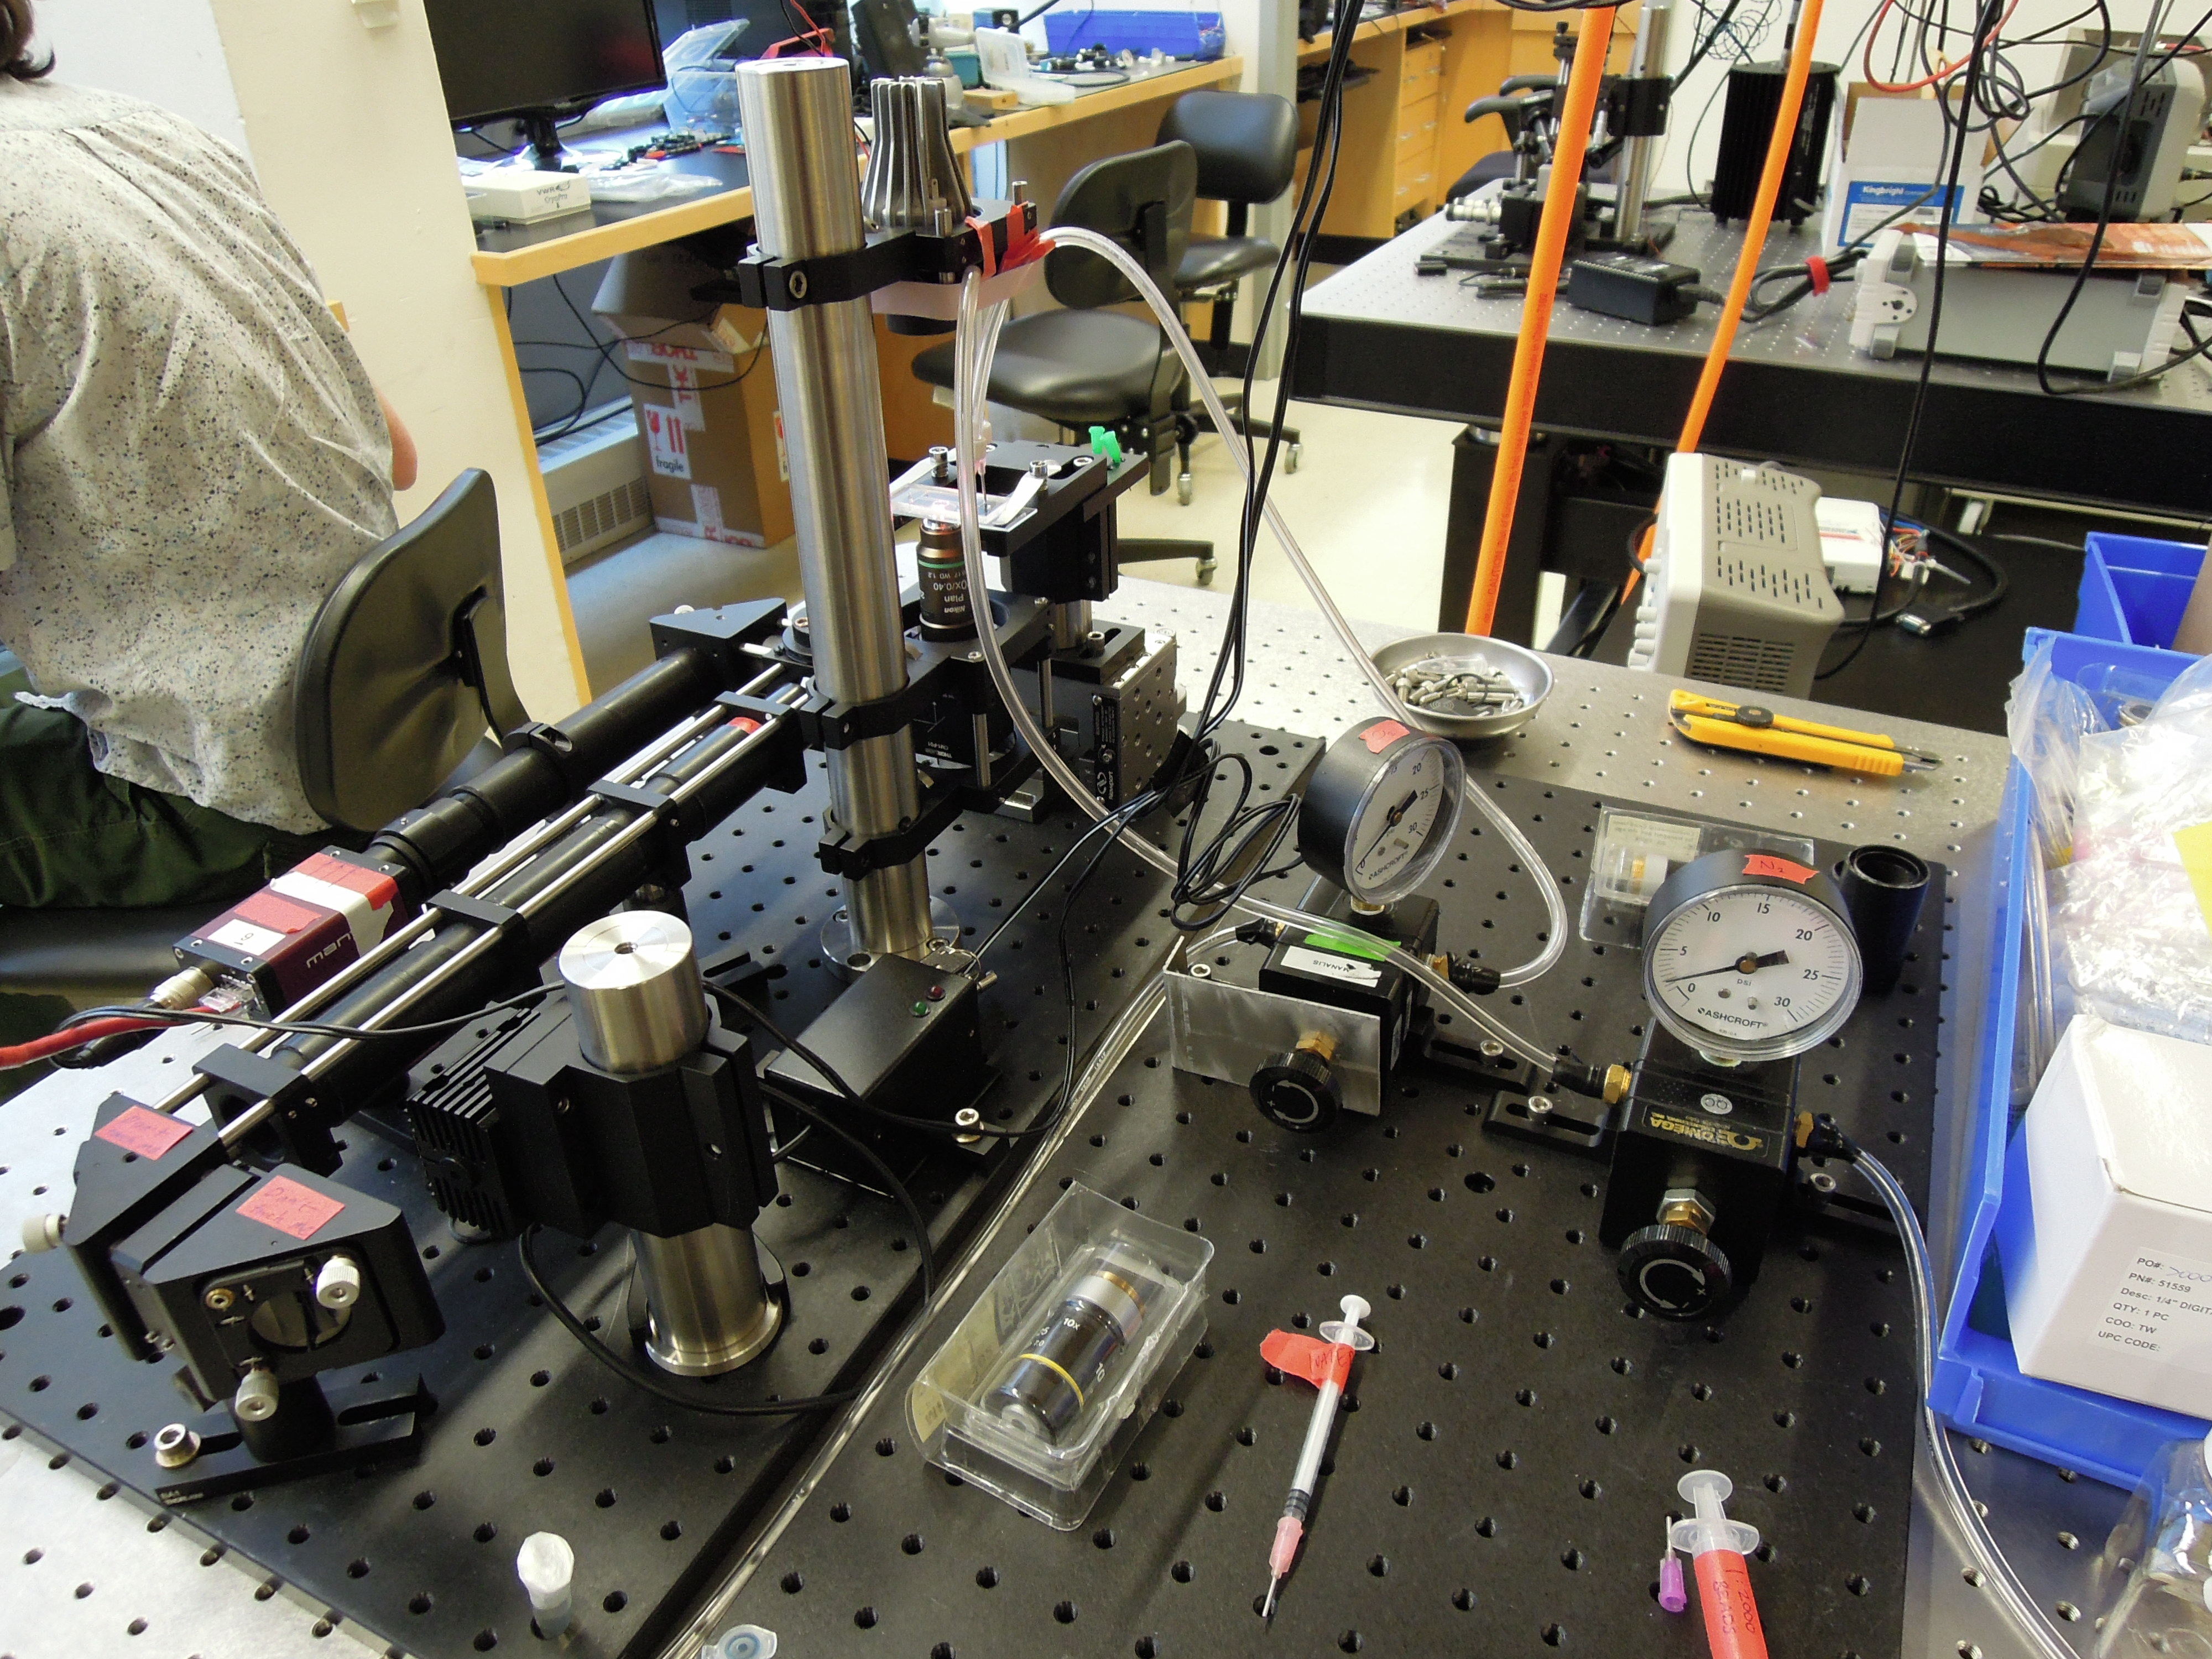
\includegraphics[width=\textwidth]{plots/Setup.jpg}
	\caption{The full experimental setup. The microfluidic device is on the stage of the microscope, which was custom-built for these experiments. The gas regulators allow for controlled flow of O\textsubscript{2} and N\textsubscript{2} gas into the device via syringe tips inserted into access holes in the device.}
	\label{fig:SetupPhoto}
\end{figure}

The aerotaxis experiments were run in a microfluidic device that contained the bacteria and the gases, nitrogen and oxygen, in parallel channels separated by thin layers of PDMS permeable to the gases. The device is located on the stage of a custom-built fluorescence microscope. A photo of the overall setup is shown in Figure \ref{fig:SetupPhoto}.

\subsection{The microscope}

\begin{figure} 
	\centering
    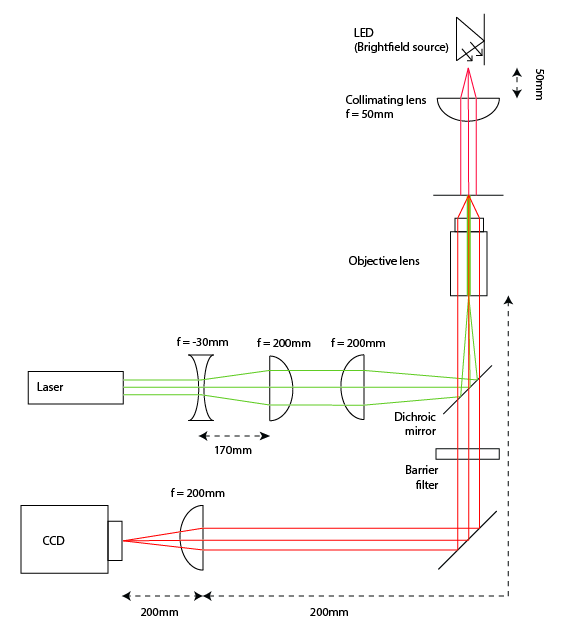
\includegraphics[width=\textwidth]{plots/MicroscopeDiagram.png}
	\caption{The fluorescence path (green), brightfield light source, and imaging path (red) of the microscope used to capture data from the microfluidic device with a CCD camera.}
	\label{fig:MicroscopeDiagram}
\end{figure}

The microscope used for the project is a standard 4f microscope with 200mm Nikon objectives. The objective is mounted inverted to facilitate access to the sample. 10X and 20X objectives were used to collect micrographs during the course of the experiments. Brightfield illumination is provided by a red LED and collimated by a small lens. A barrier filter filters out other illumination from the CCD. These components are shown in  Figure \ref{fig:MicroscopeDiagram}.

A fluorescence pathway was also built to aid in cell tracking. The fluorescence illumination is provided by a 532 nm green laser source, which is expanded and then focused onto the surface of the objective in order to produce a collimated beam on the sample. A dichroic mirror reflects laser light onto the sample while allowing light emitted by fluorescence to pass through to the CCD.

Calibration was done optically using an Air Force Microscope Target and an image capture program to verify the magnification. The magnification was calculated from measurements of the pixels in a photograph of a known distance and the dimensions of the imager in the CCD, .

\subsection{The microfluidic device} % Logan or Kiarash?

\begin{figure} 
	\centering
    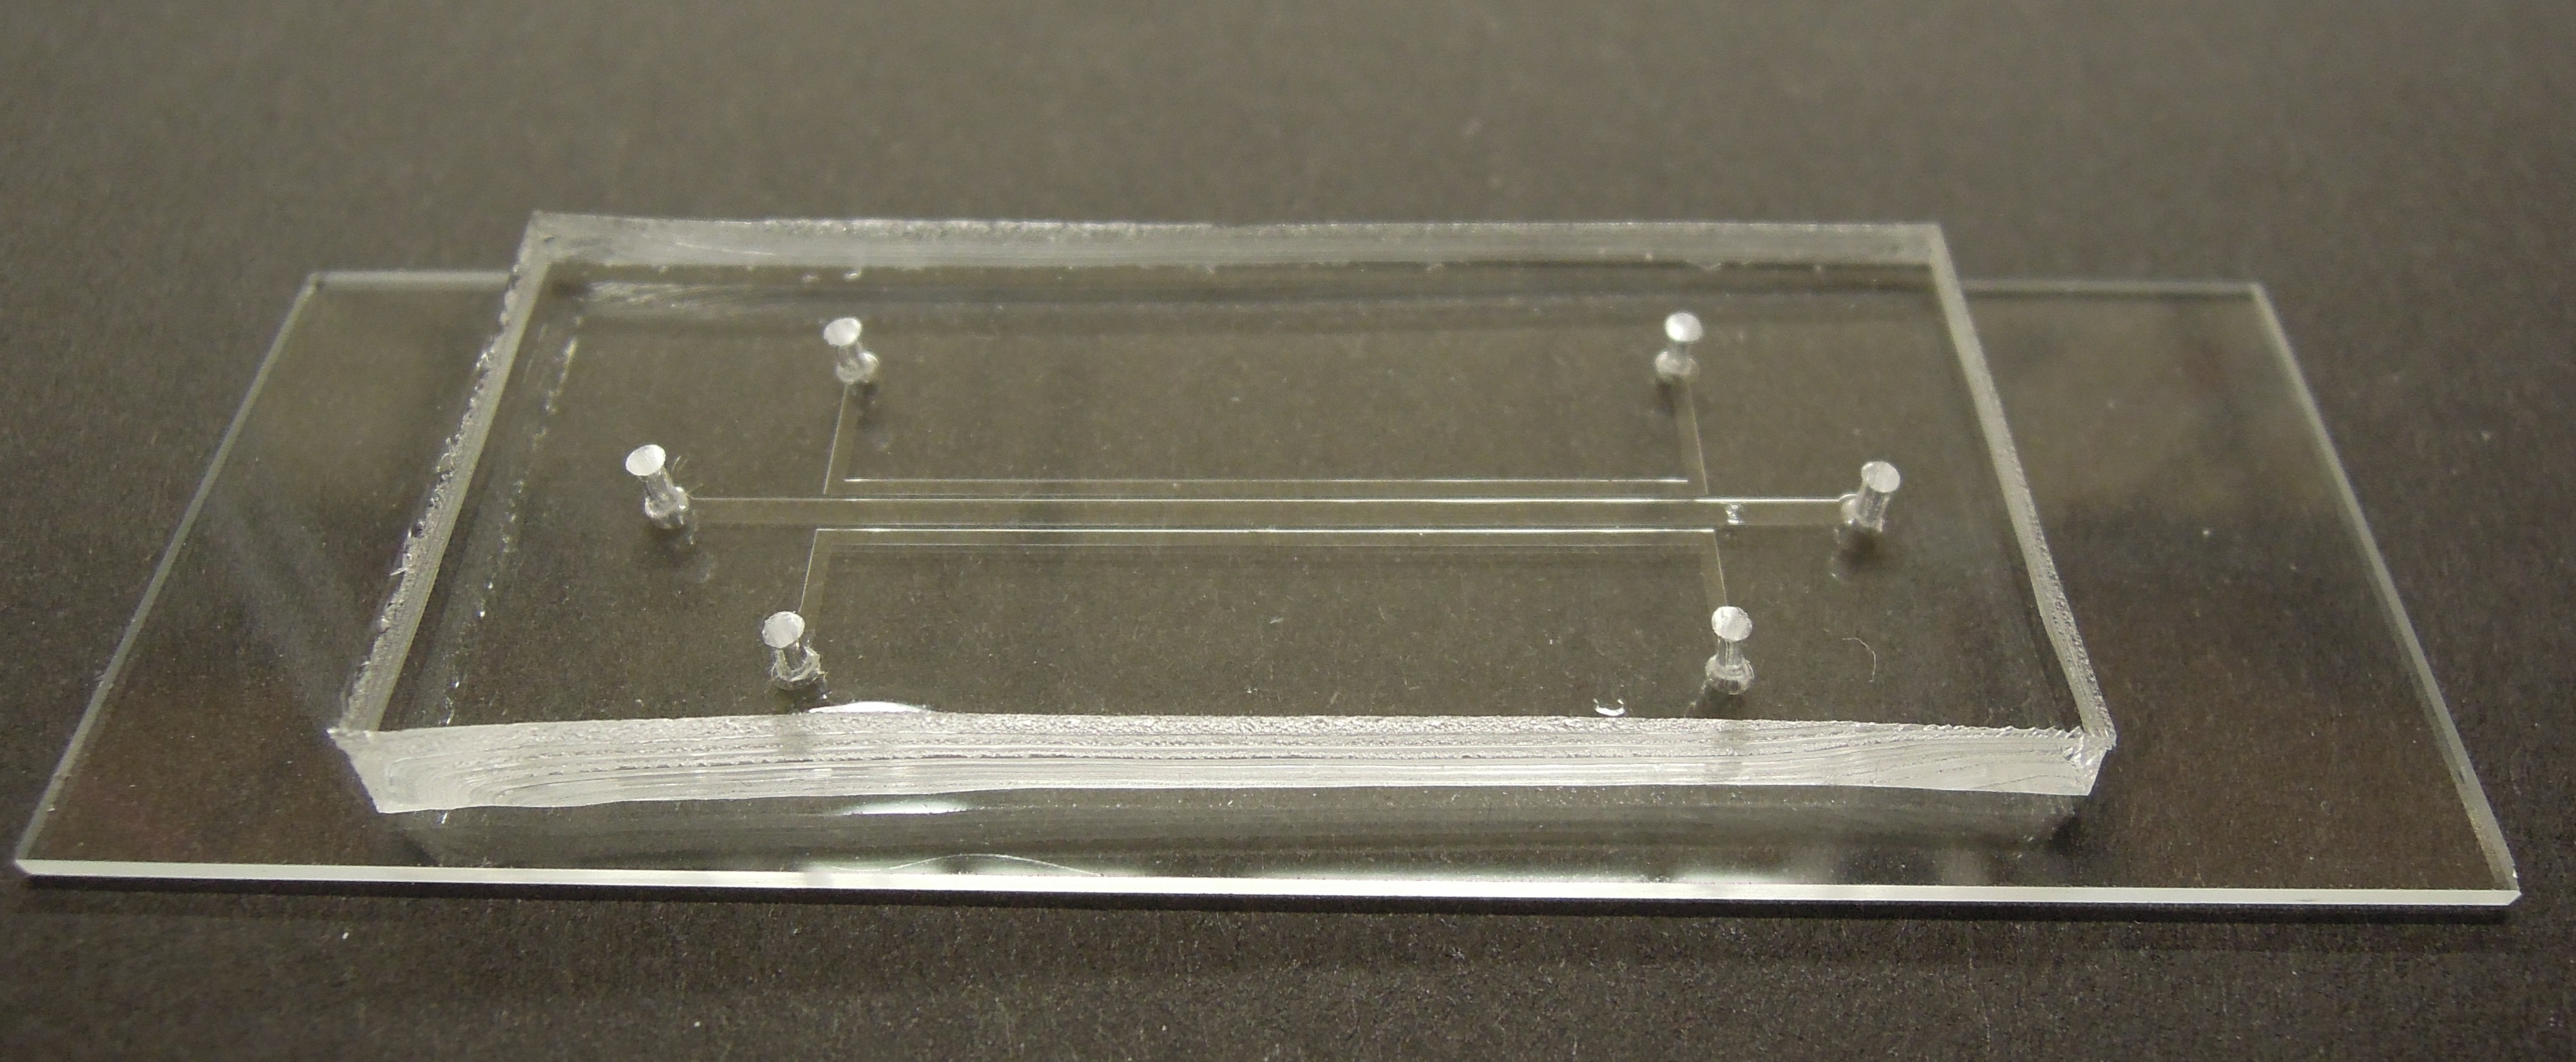
\includegraphics[width=\textwidth]{plots/Device.jpg}
	\caption{The microfluidic device. It is composed of PDMS, a silicone-like polymer, and features 3 channels parallel to each other. The center channel holds the bacteria; the two outer channels, thinner than the bacteria channel, direct the gas flow. PDMS is gas-permeable, so the gas will diffuse into the center channel where the bacteria are located.}
	\label{fig:Device}
\end{figure}

The microfluidic device is composed of the elastomeric material Polydimethylsiloxane (PDMS). The mask, a silicon wafer obtained from the MIT Environmental Microfluidics Group, was used in conjunction with UV-curing photopolymers to create a master mold for the PDMS devices. PDMS and its curing agent were mixed in a 10:1 ratio, respectively, and poured over the mold in a dish. The dish was degassed in a vacuum chamber and then cured for approximately 12 hours. After the PDMS had cured, the excess around the device was cut away, yielding the rectangular shape shown in Figure \ref{fig:Device}, and 0.050'' holes were punched through the device to allow access to the ends of each channel. After the device was completed, one side was treated with oxygen plasma, and it was bonded to a glass slide.

The device has three parallel channels formed by indentations in the PDMS; the glass slide creates the fourth wall of each channel, closing them. Each channel is 600 microns wide and 50 microns deep, with 200 microns of separation between each channel. Bacteria was injected into the center channel and allowed to settle before data collection began. Oxygen and nitrogen flows were directed down the outside channels. The devices were cleaned with isopropanol, which does not degrade the PDMS or the plasma bond, and reused for multiple experiments.

\subsection{Gas flow} % Kat?

\begin{figure} 
	\centering
    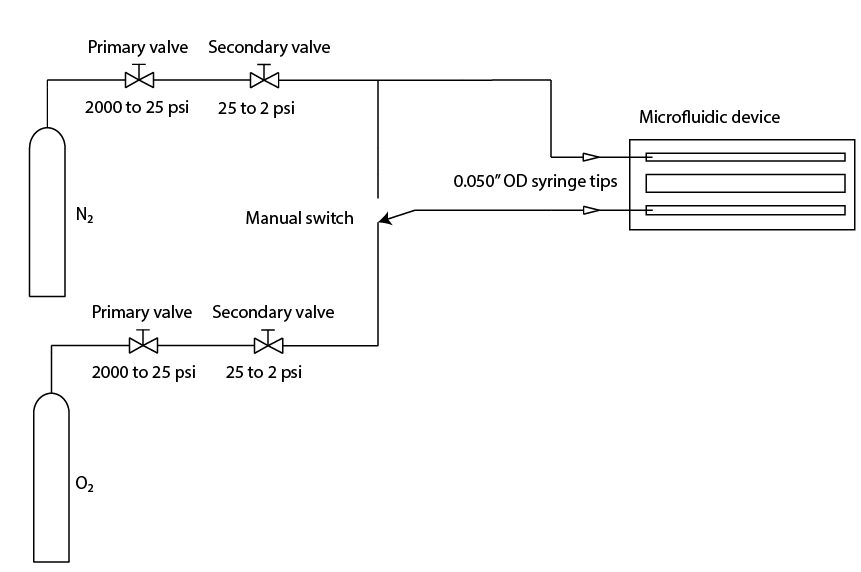
\includegraphics[width=\textwidth]{plots/GasFlow.png}
	\caption{The gas flow path, from the cylinders to the microfluidic device, which ultimately exhausts to air. The gas lines switch, providing N\textsubscript{2} to one microfluidic gas channel and either N\textsubscript{2} or O\textsubscript{2} to the other gas channel, depending on the experiment phase.}
	\label{fig:GasFlow}
\end{figure}

The essence of aerotaxis is the gas gradient to which bacteria respond. The gas gradient was achieved by routing oxygen and nitrogen through the outside microfluidic channels parallel to the bacteria channel. Both gases originate in storage cylinders attached to primary regulators. These regulators drop the gas pressure from 2000 psi to 25 psi. After exiting the primary regulator, each gas flows through 1/8'' ID Tygon E-3603 tubing to a secondary regulator that drops the pressure further, providing 2 psi to the lines connected to the device.

These lines have two different configurations during the experiment, providing either N\textsubscript{2} to one microfluidic gas channel and O\textsubscript{2} to the other, or providing N\textsubscript{2} to both microfluidic gas channels. These configurations are shown in Figure \ref{fig:GasFlow} as a switch. Two lines of tubing interface with the device via Luer lock fittings attached to 0.050'' OD syringe tips that mate with 0.059'' ID access holes in the PDMS. One of these two lines is permanently connected to the nitrogen flow through a T-junction. The other line switches between the T-junction and the secondary O\textsubscript{2} regulator, depending on the experiment phase.  The gases flow through the device, diffusing into the PDMS to reach the bacteria chamber, and ultimately exhaust to the environment through the access holes at the channels� other ends.

\subsection{Bacteria culturing} % Brian?
\section{Results} % all of us

Relevant plots and micrographs, as well as the experimental methods and data processing that produced them, are displayed and explained on the subsequent pages.

\begin{figure}[p!] 
  \centering
    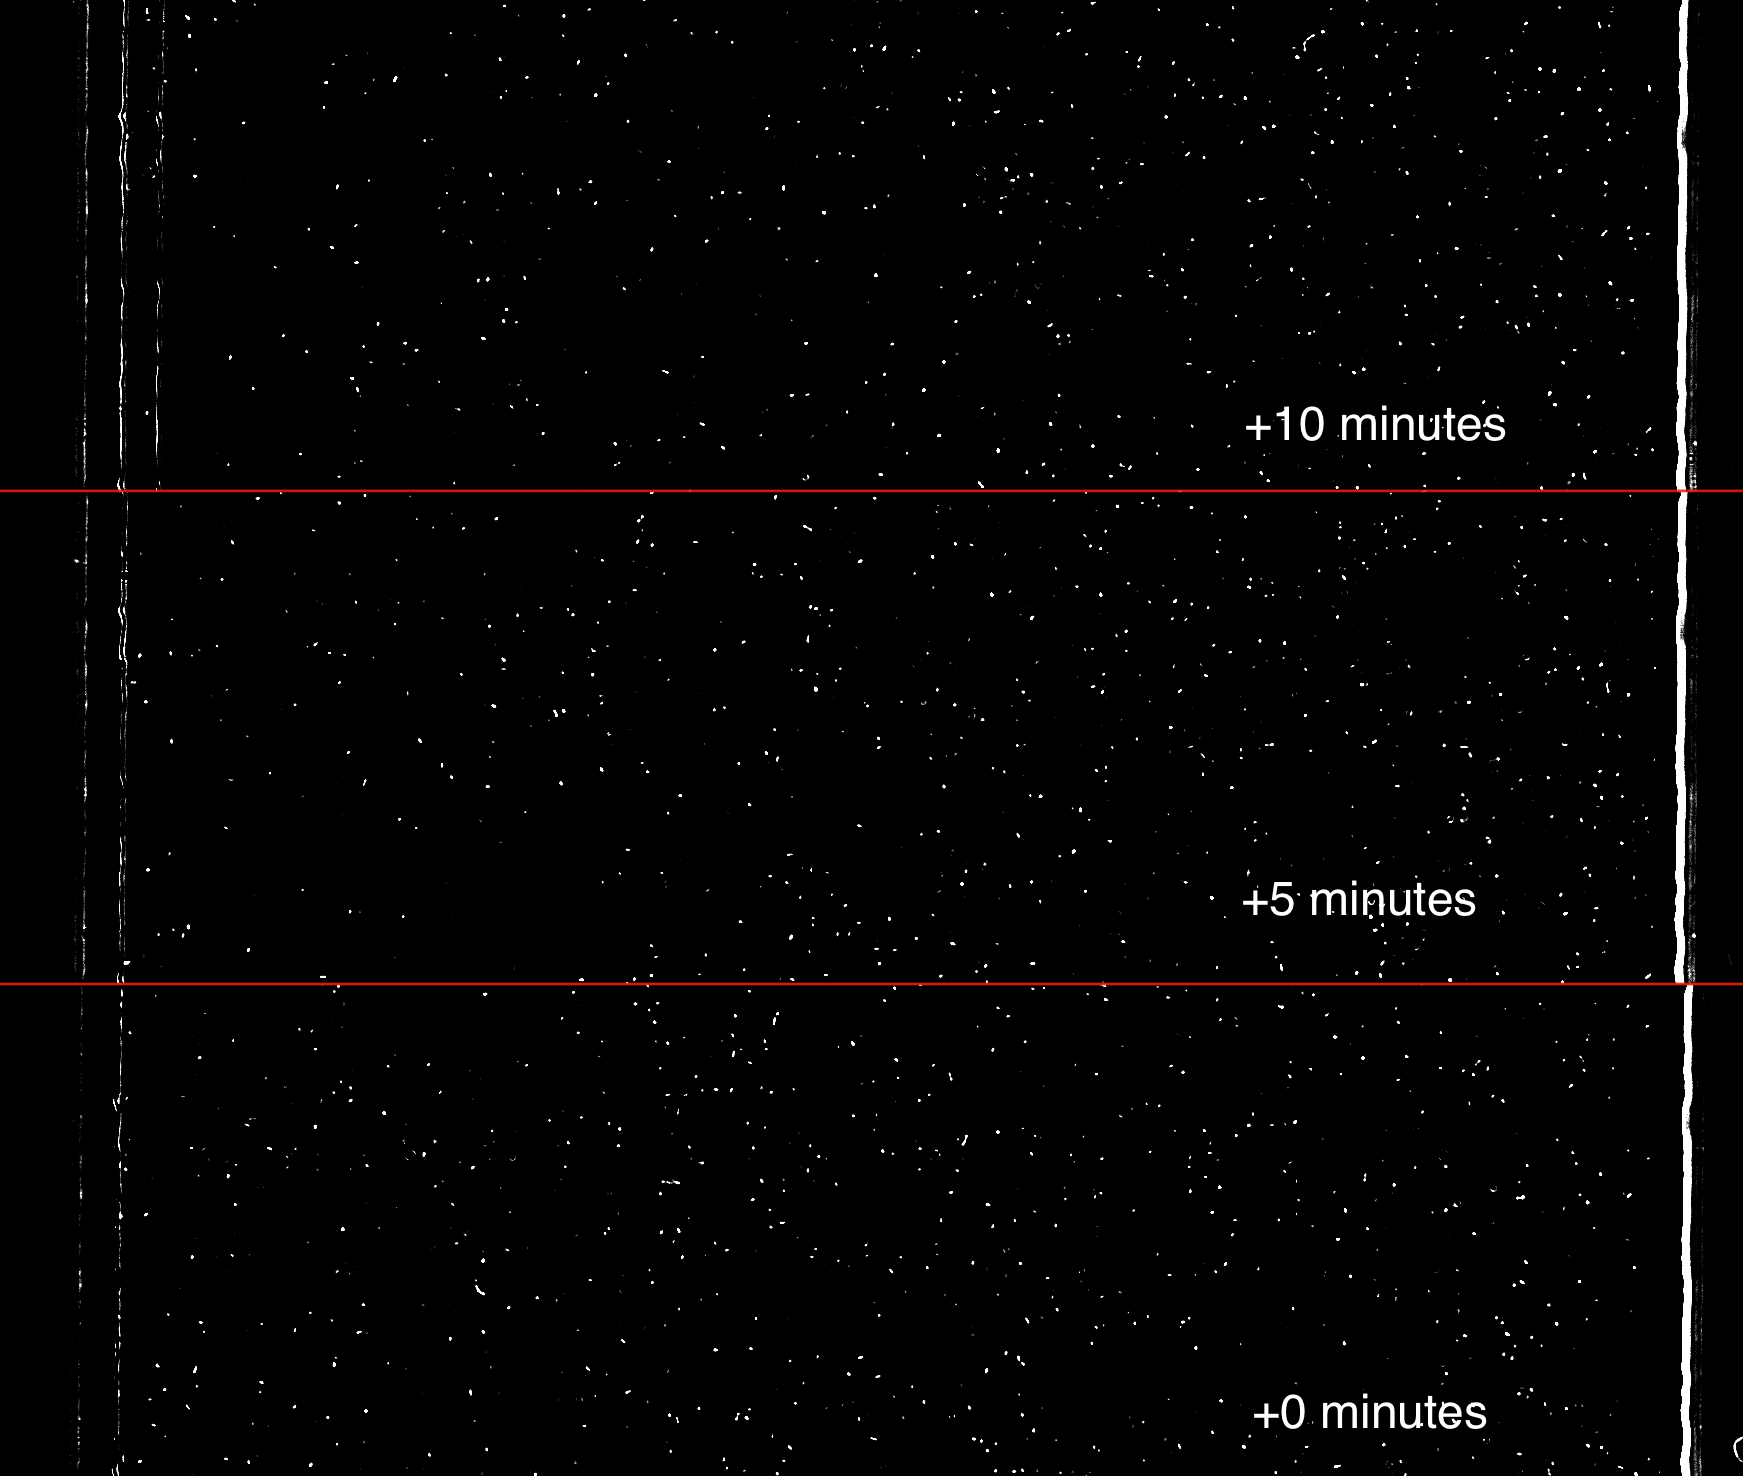
\includegraphics[width=\textwidth]{plots/contrast.png}
      \caption[Visual verification of aerotaxis]{This micrographic ``panorama'' shows the entire width of the center channel, thresholded to highlight bacteria. Note that prior to flowing oxygen and nitrogen, the bacteria are evenly distributed in the channel. 5 minutes after gas flow began, bacteria have begun to accumulate on the oxygenated side of the channel (the right hand side). \\
      
      This experiment was conducted by placing bacteria in the channel and taking several micrographs across the channel, then combining them and performing thresholding in Adobe Photoshop. The process was repeated 5 minutes and 10 minutes after gas flow started.}
      \label{fig:gradient}
\end{figure}

\begin{figure}[p!] 
  \centering
    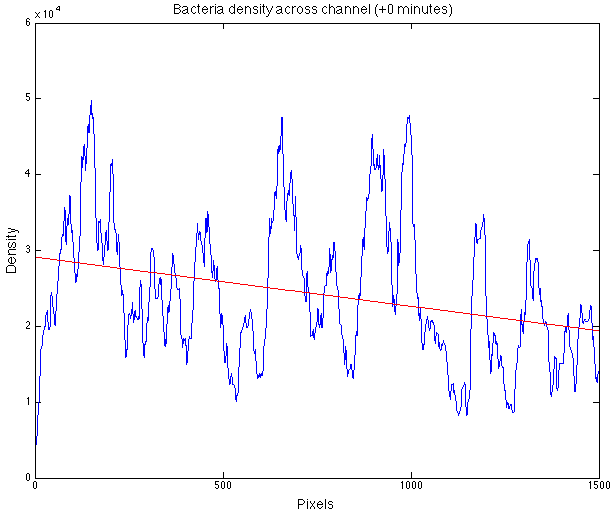
\includegraphics[width=0.49\textwidth]{plots/0min_new.png}
     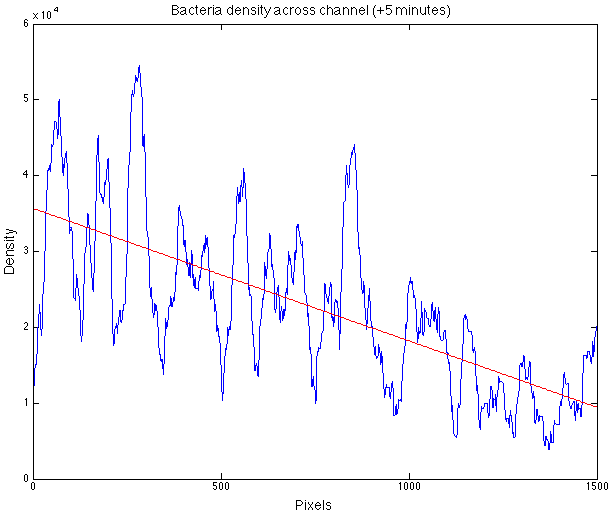
\includegraphics[width=0.49\textwidth]{plots/5min_new.png}
    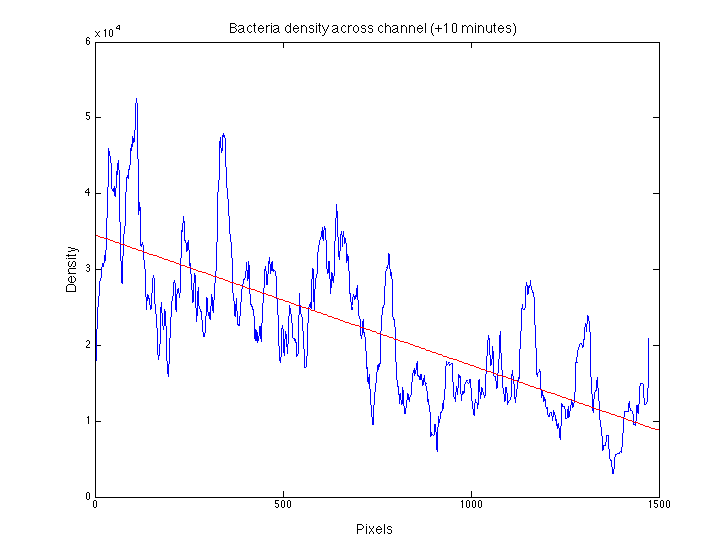
\includegraphics[width=0.49\textwidth]{plots/10min_new.png}

      \caption[Quantitative verification of aerotaxis]{These plots represent the same data as the panorama in Figure \ref{fig:gradient}, showing the density of bacteria laterally across the channel, prior to gas flow, 5 minutes after gas flow, and 10 minutes after gas flow. This shows that the gradient (the slope of the linear fit line) increases with time.\\
      
      These plots were produced from the panoramic image by summing each column in MATLAB, convolving with a rectangle function to smooth out discrete impulses, and using MATLAB to compute a linear fit.}
\end{figure}

\begin{figure}[p!] 
  \centering
    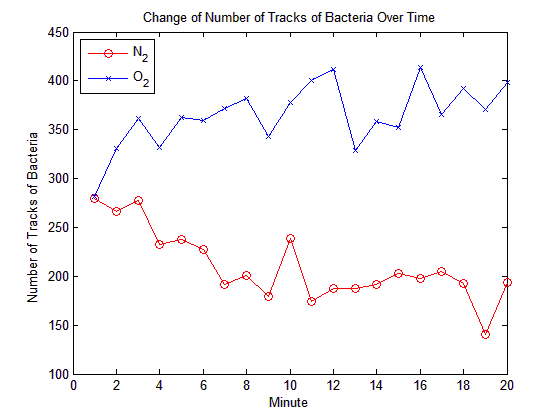
\includegraphics[width=\textwidth]{plots/number_Tracks.png}
      \caption[Number of trackable bacteria]{The number of trackable bacteria adjacent on the nitrogen side of the channel as compared to the number on the oxygen side. \\
      
      This plot was produced by finding bright centroids in captured microscope frames, and tracking the motion of the centroids. The number of ``tracks'' produced corresponds to the number of trackable bacteria. \\
      
      This experiment was conducted by placing bacteria in the center channel, running gas through the outer channels, and taking 30 sequential frames (at 15 fps), every minute, on both sides of the channel.}
\end{figure}

\begin{figure}[p!] 
  \centering
    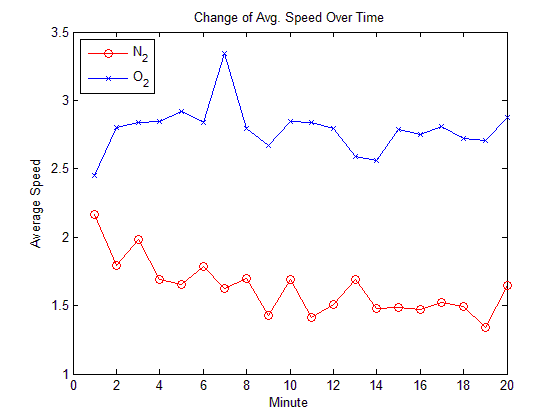
\includegraphics[width=\textwidth]{plots/average_speed.png}
      \caption[Speed of trackable bacteria]{The speed of trackable bacteria adjacent to the nitrogen side of the channel as compared to the number on the oxygen side. The large spike at 7 minutes is due to the table being bumped, creating drift -- this error source is discussed later in the report.\\
      
      This plot was produced by finding bright centroids in captured microscope frames and tracking the motion of the centroids. The distance moved by each bacteria  ``track'' was averaged every minute (for each sequence of 30 frames). \\
      
            This experiment was conducted by placing bacteria in the center channel, running gas through the outer channels, and taking 30 sequential frames (at 15 fps), every minute, on both sides of the channel.}
\end{figure}

\begin{figure}[p!] 
  \centering
    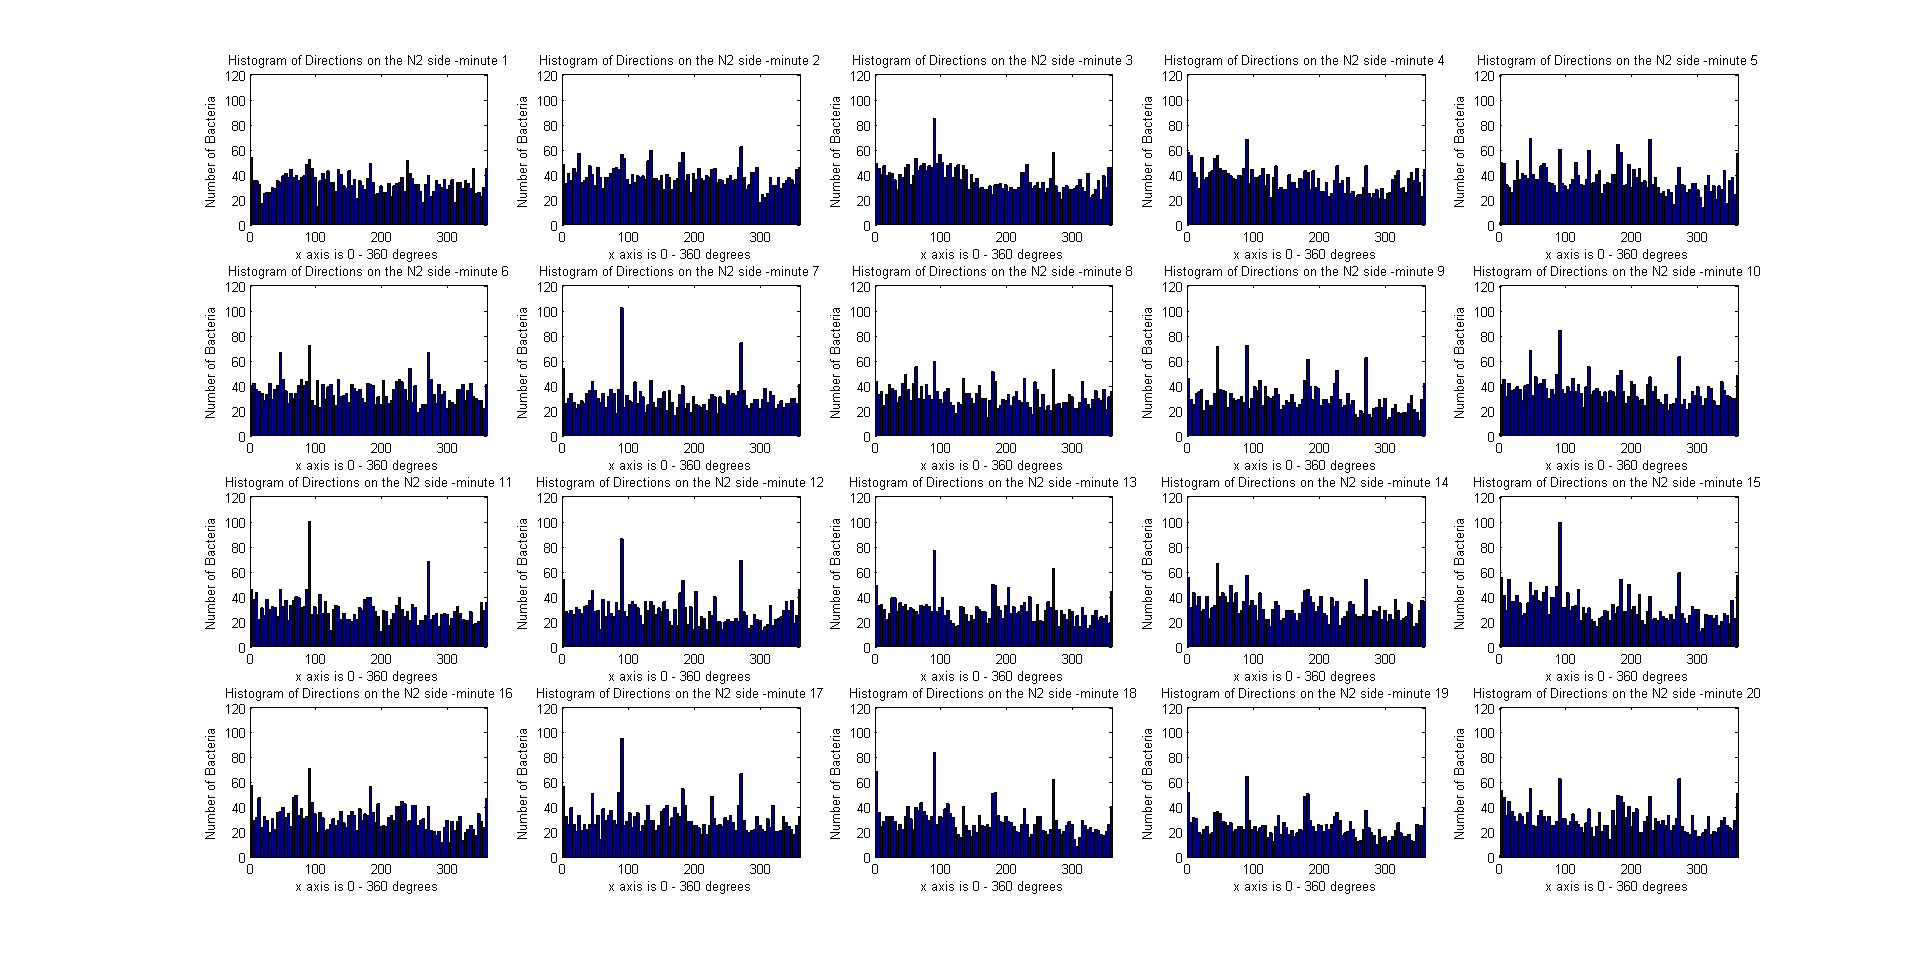
\includegraphics[width=0.9\textwidth]{plots/directions_hist_N2.png}
    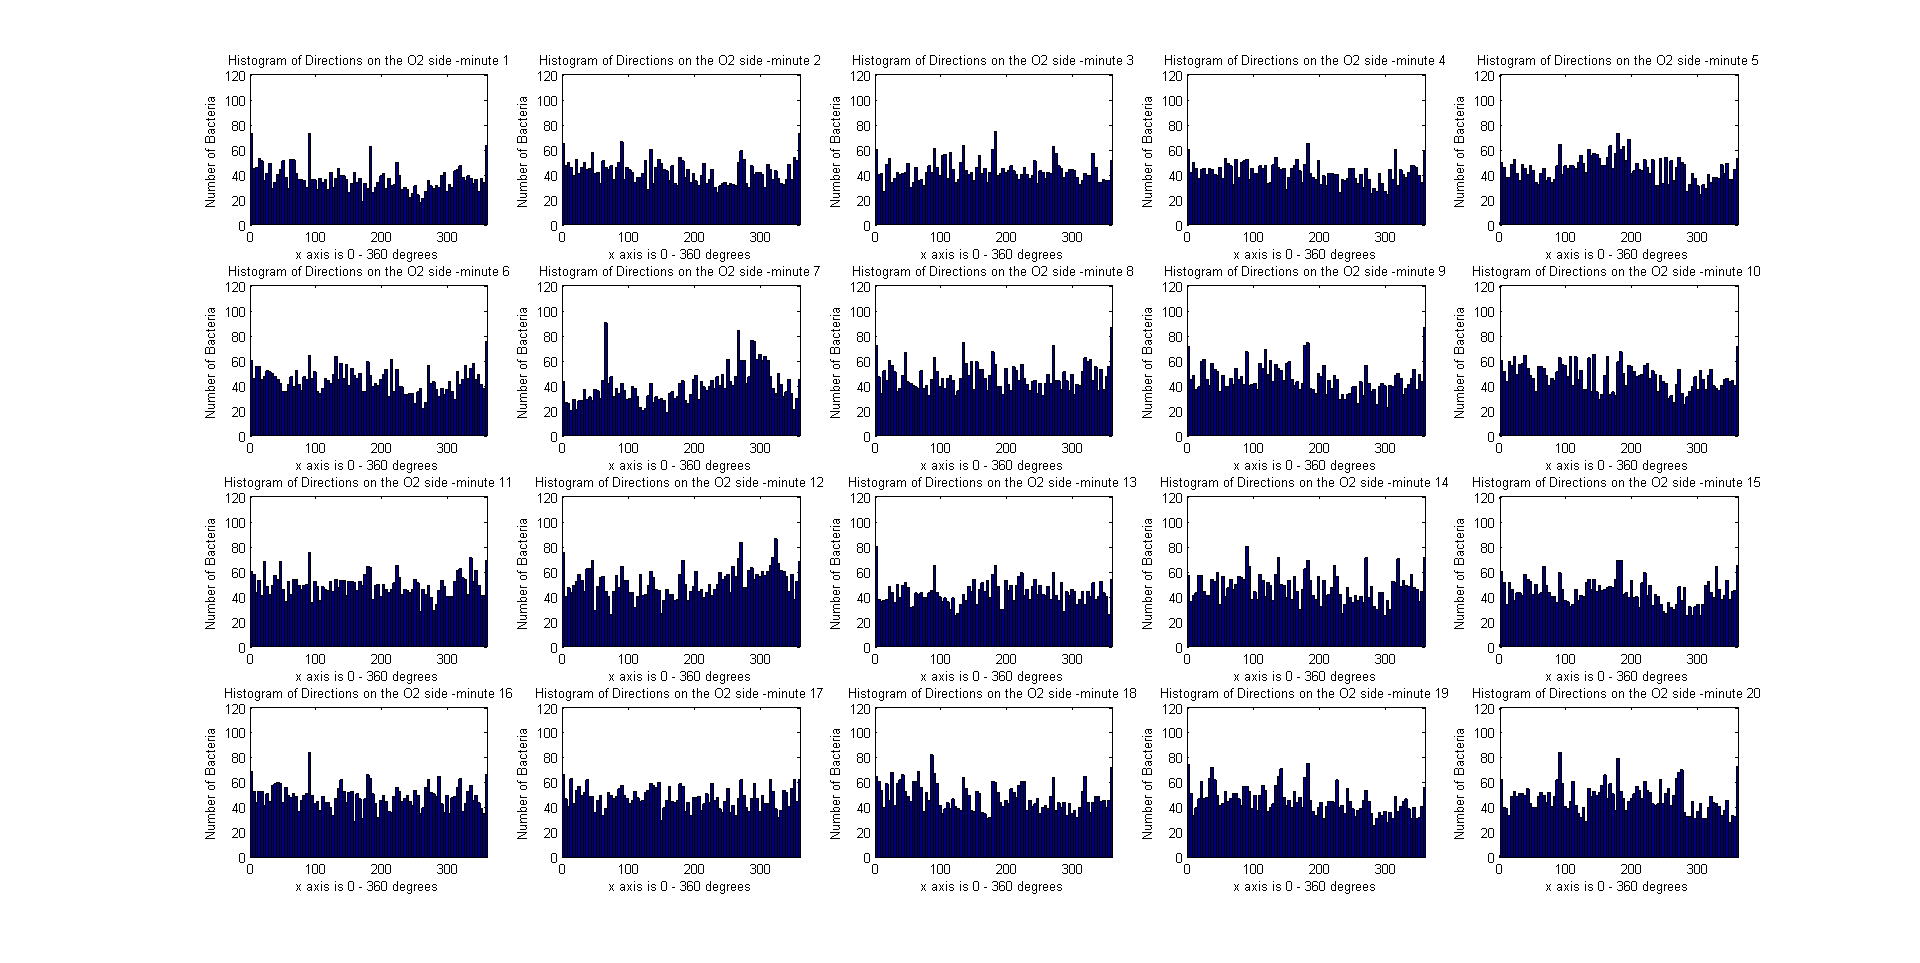
\includegraphics[width=0.9\textwidth]{plots/directions_hist_O2.png}    
      \caption[Histogram of direction of movement]{Histograms of direction of movement of bacteria on the nitrogen side of the channel (top) and on the oxygen side (bottom). Note that there is no discernible trend towards a particular direction in either case. \\
      
      This plot was produced by finding bright centroids in captured microscope frames and tracking the motion of the centroids. These ``tracks'' were analyzed to find the direction of movement of each bacteria from frame to frame. This list of directions of movement was then plotted as a histogram for each minute (30 frames) of captured data. \\
      
            This experiment was conducted by placing bacteria in the center channel, running gas through the outer channels, and taking 30 sequential frames (at 15 fps) every minute on both sides of the channel.}
\end{figure}

\begin{figure}[p!] 
  \centering
    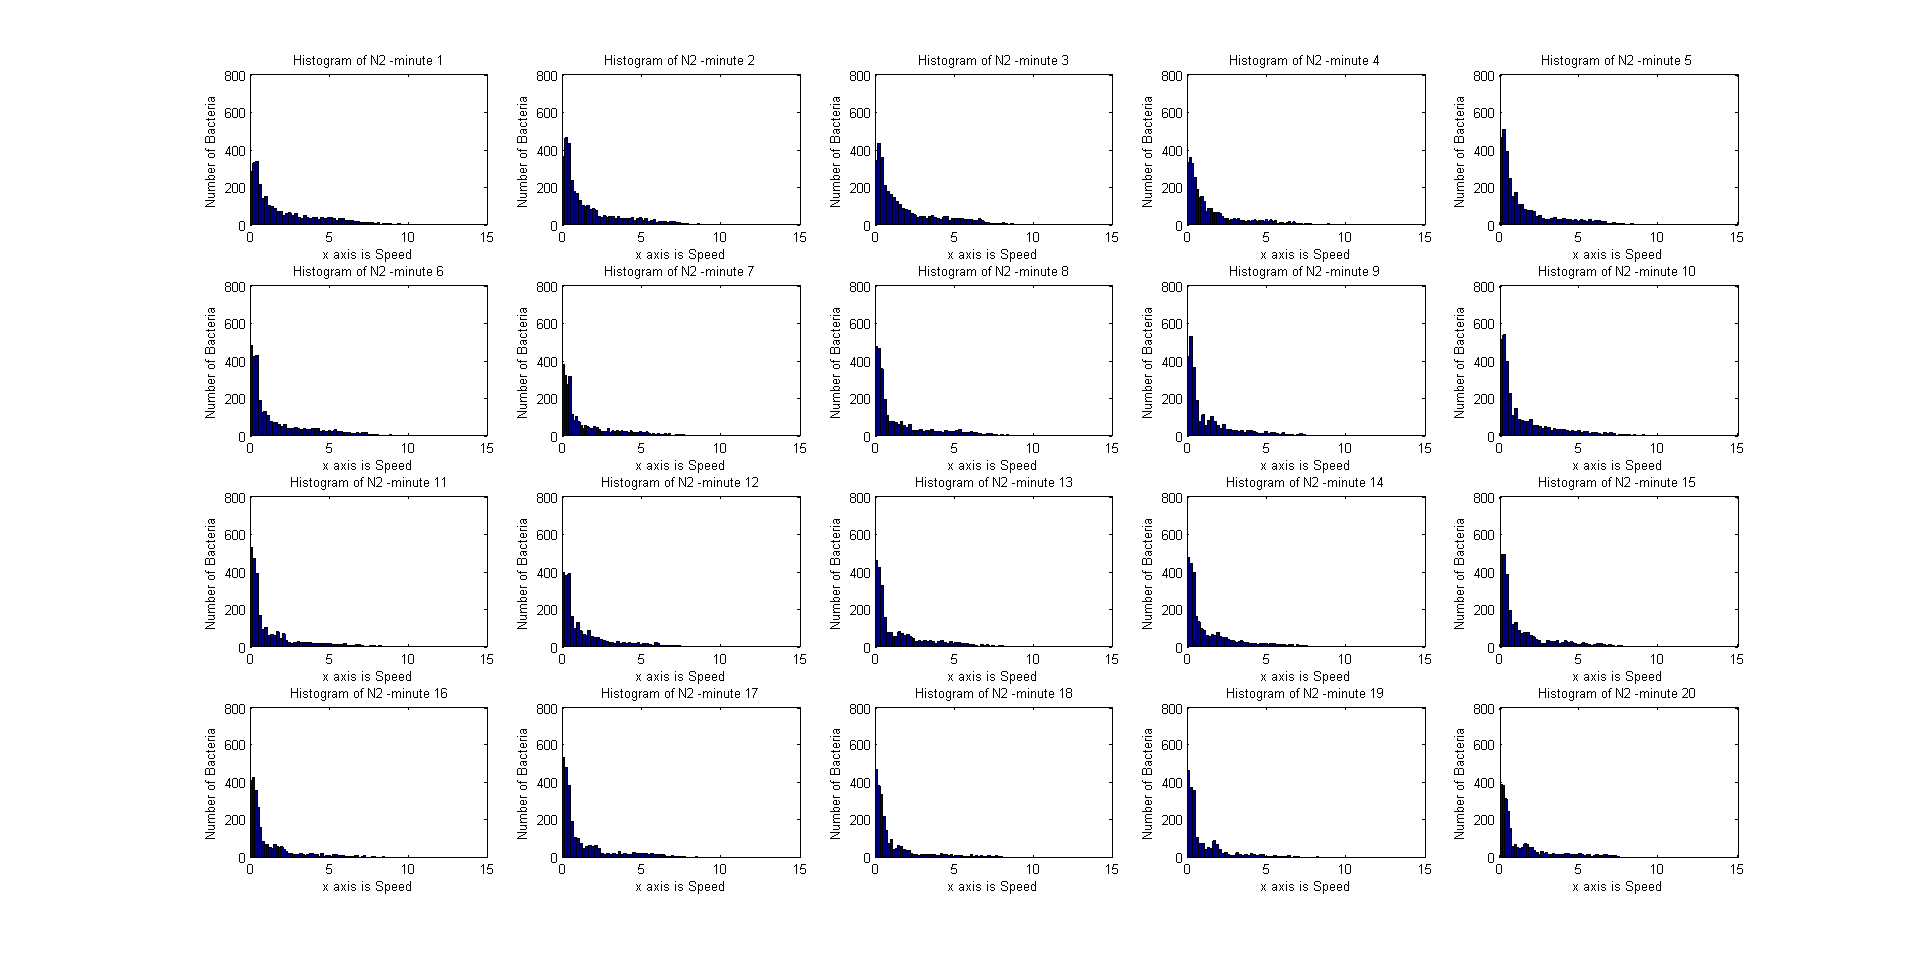
\includegraphics[width=0.86\textwidth]{plots/histograms_N2.png}
    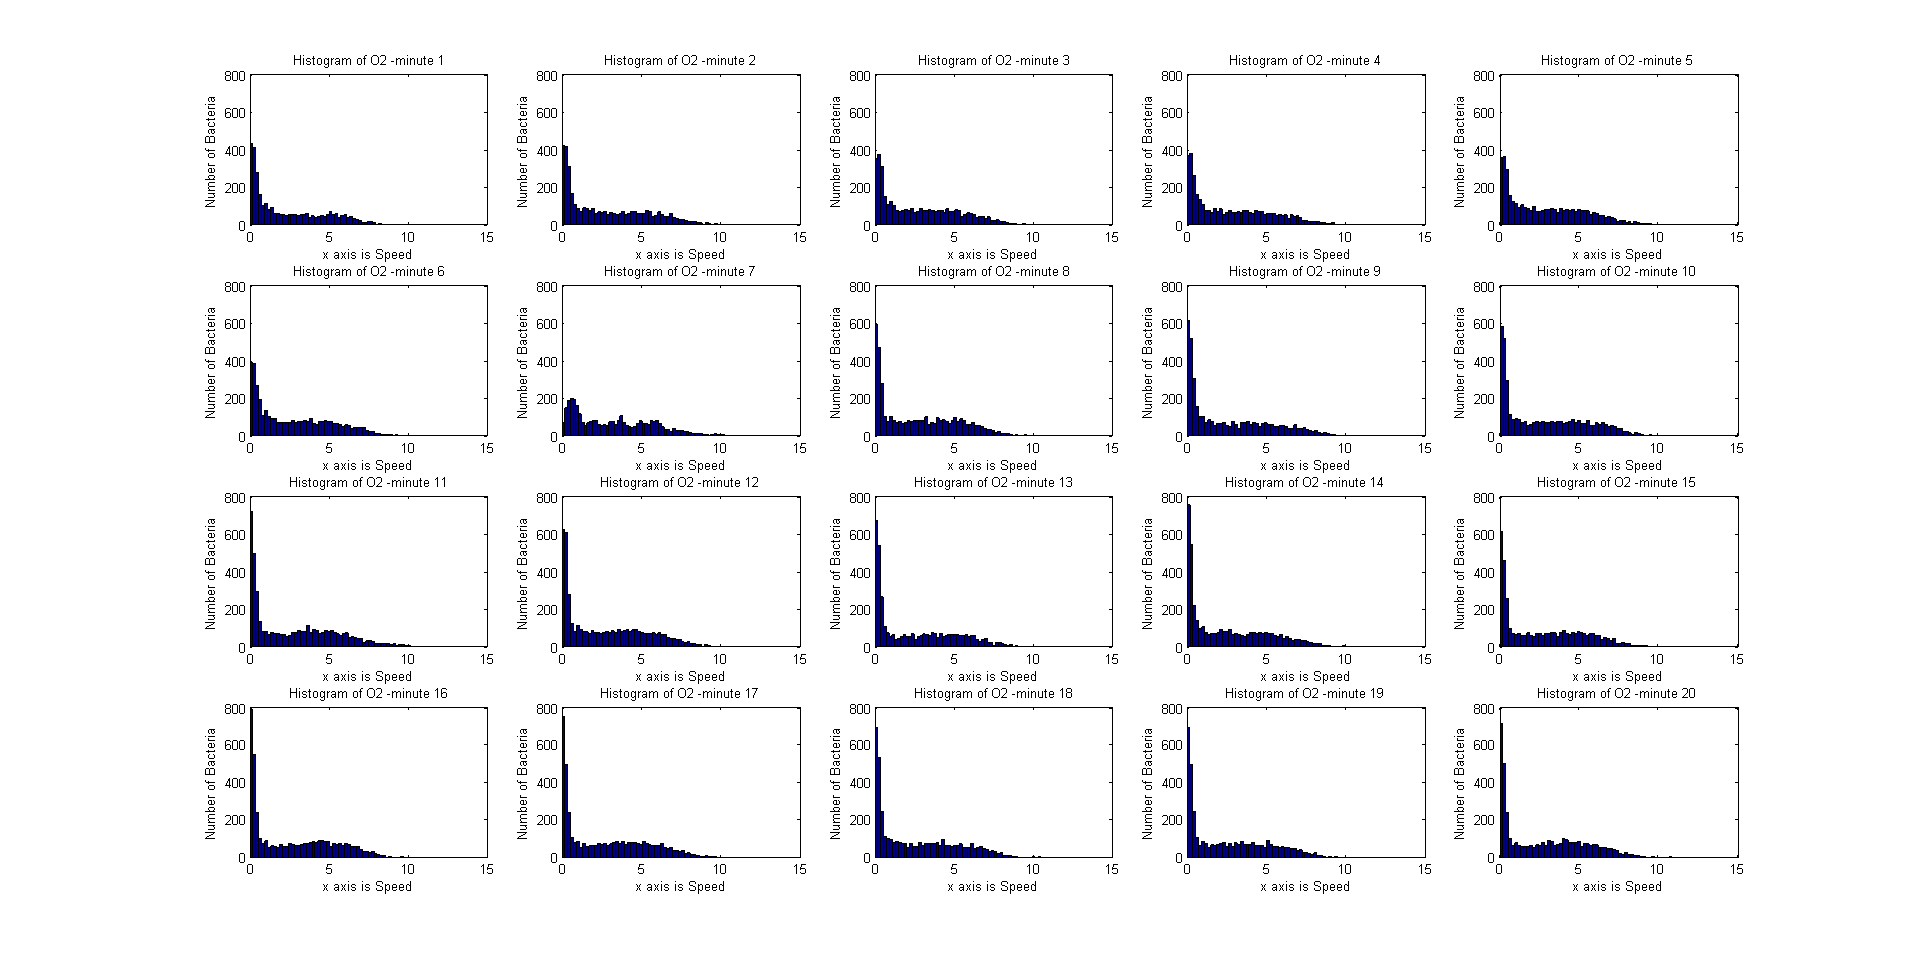
\includegraphics[width=0.86\textwidth]{plots/histograms_O2.png}    
      \caption[Histogram of speed of movement]{Histograms of speed of bacterial movement on the nitrogen side of the channel (top) and on the oxygen side (bottom). Note that there is no discernible change over time in either case. Note also that a significant number of bacteria have speeds very close to zero. This is due to the ``stickiness'' of PDMS, a problem which was later rectified by coating the PDMS channel in bovine serum albumin (BSA), which acts to lubricate the channel. \\
      
      This plot was produced by finding bright centroids in captured microscope frames and tracking the motion of the centroids. These ``tracks'' were analyzed to find the average speed of movement of each bacteria from frame to frame. This list of directions of movement was then plotted as a histogram for each minute (30 frames) of captured data. \\
      
            This experiment was conducted by placing bacteria in the center channel, running gas through the outer channels, and taking 30 sequential frames (at 15 fps) every minute on both sides of the channel.}
\end{figure}

\begin{figure}[p!] 
  \centering
    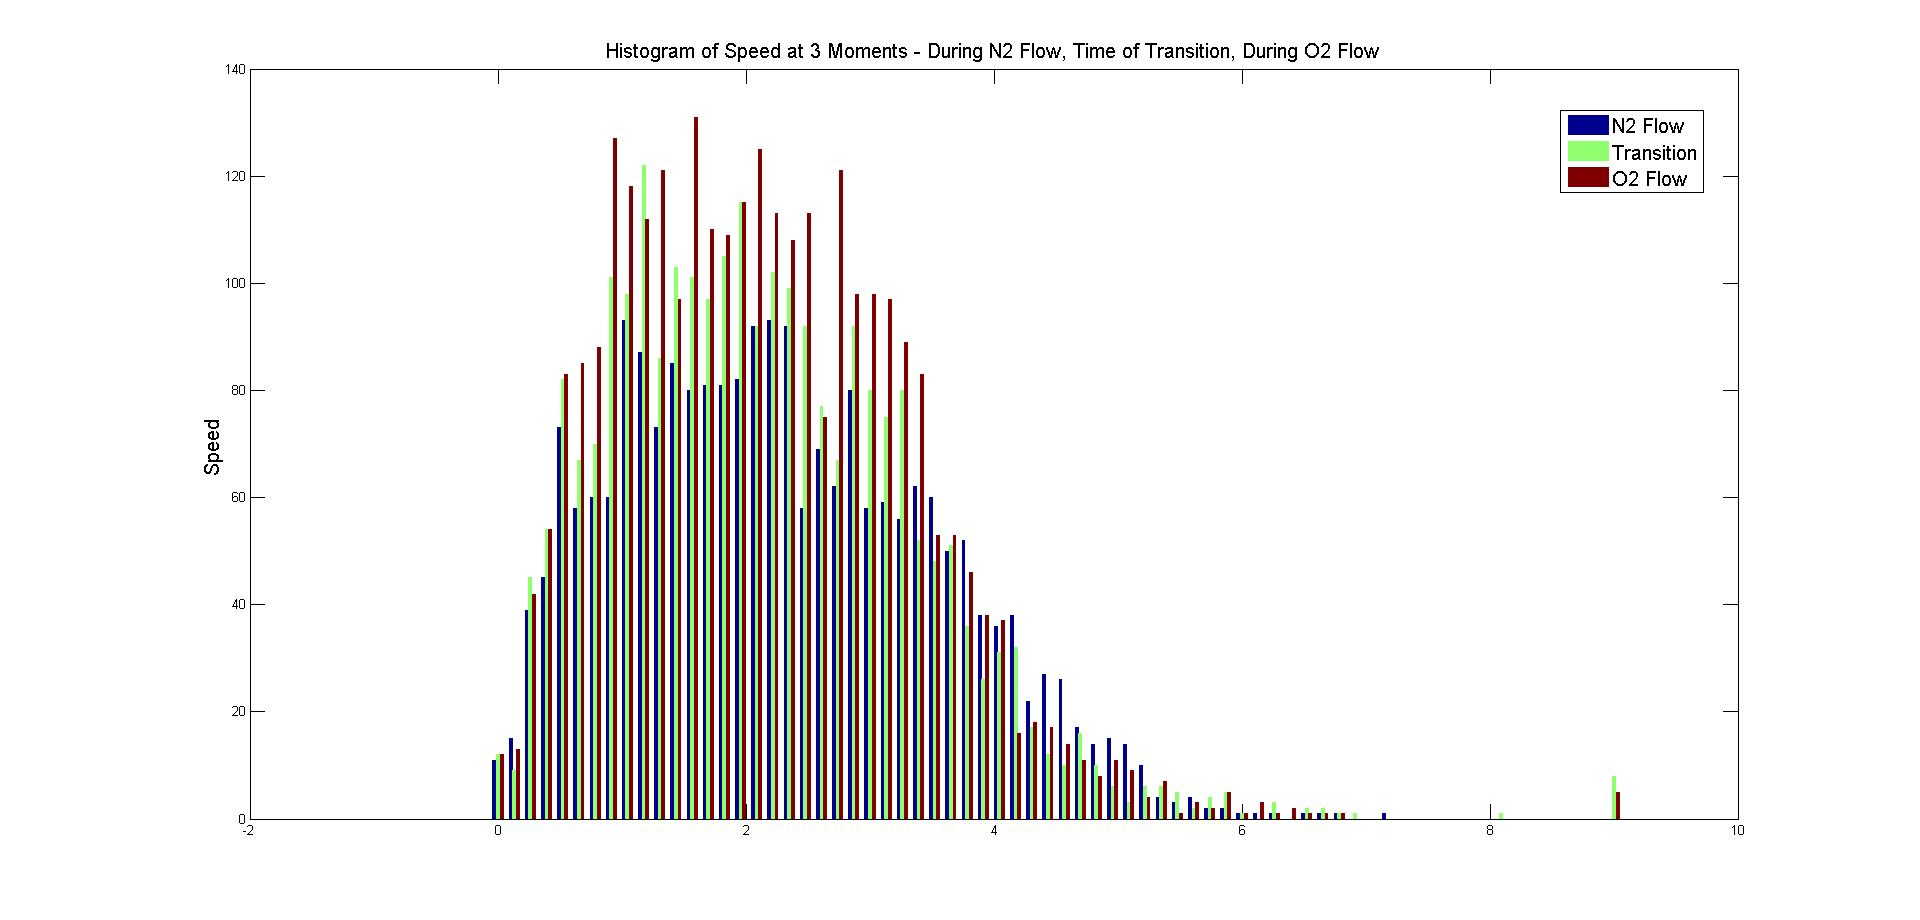
\includegraphics[width=\textwidth]{plots/speed_histogram.jpg}
      \caption[Histogram of bacteria speed]{The distribution of  speed of bacteria in a channel coated with BSA, at three points in time --- while flowing nitrogen through both gas channels, while flowing nitrogen through one gas channel and oxygen through the other, and while transitioning between the two flows.\\
      
      This plot was produced by finding bright centroids in captured microscope frames and tracking the motion of the centroids. A histogram was produced of the distribution of the amount of movement of each bacteria between subsequent frames. \\
      
            This experiment was conducted by placing bacteria in the center channel, and starting a flow of nitrogen through both outer channels. A sequence of 30 frames was taken, at 15 fps, in the center of the channel. This was repeated every 15 seconds for approximately 10 minutes before one of the nitrogen gas lines was switched to oxygen; the experiment continued for another 10 minutes.}
\end{figure}

\begin{figure}[p!] 
  \centering
    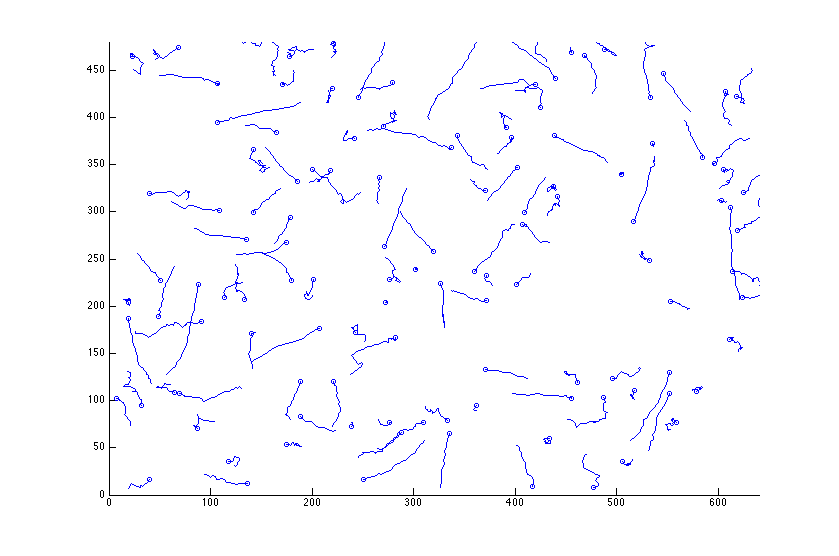
\includegraphics[width=0.5\textwidth]{plots/tracks_1.png}
    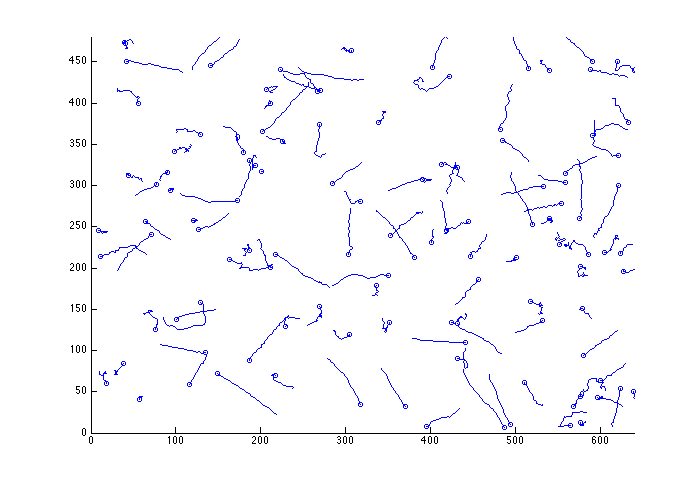
\includegraphics[width=0.5\textwidth]{plots/tracks_2.png}
    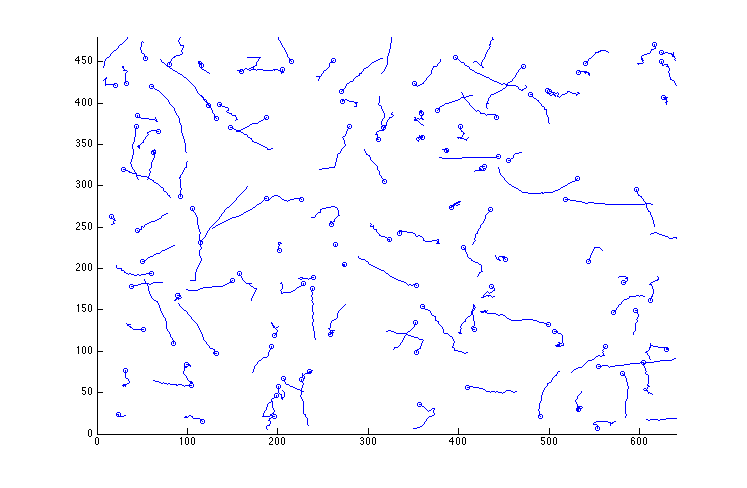
\includegraphics[width=0.5\textwidth]{plots/tracks_3.png}
      \caption[Representative traces]{Representative traces of bacteria motion. \\
      
      These plots were produced by finding bright centroids in captured microscope frames and finding centroids in sequential frames that are likely to belong to the same bacteria. These are plotted prior to gas flow switch, just after gas flow switch, and several minutes after gas flow switch. No difference is apparent visually.}
\end{figure}

\begin{figure}[p!] 
  \centering
    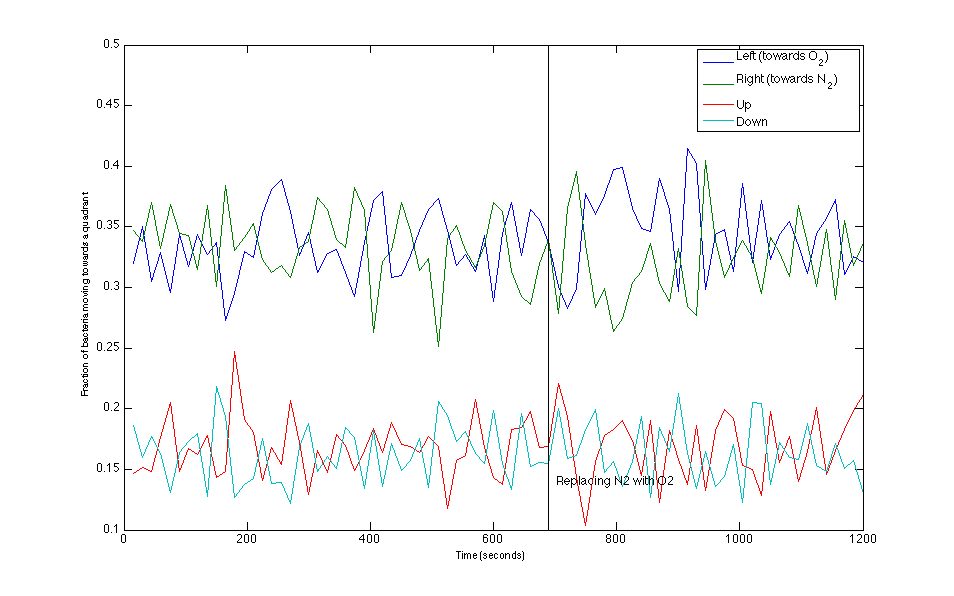
\includegraphics[width=\textwidth]{plots/direction.png}
      \caption[Bacterial motion]{Motion of motile bacteria divided into four quadrants: left (towards oxygen), right (towards nitrogen), up, and down. This shows data from one representative experiment. \\
      
      This graph was produced by calculating the distance traveled and direction of travel for every bacteria ``track'' in each sequence of 30 frames. Bacteria that moved a significant amount were considered ``motile''; all other bacteria were discarded. The bacteria were divided by  categorizing their motion into the four previously mentioned quadrants. \\
      
      This experiment was conducted by placing bacteria in the center channel and starting a flow of nitrogen through both outer channels. A sequence of 30 frames was taken, at 15 fps, in the center of the channel. This was repeated every 15 seconds for approximately 10 minutes before one of the nitrogen gas lines was switched to oxygen; the experiment continued for another 10 minutes.}
\end{figure}

\begin{figure}[p!] 
  \centering
    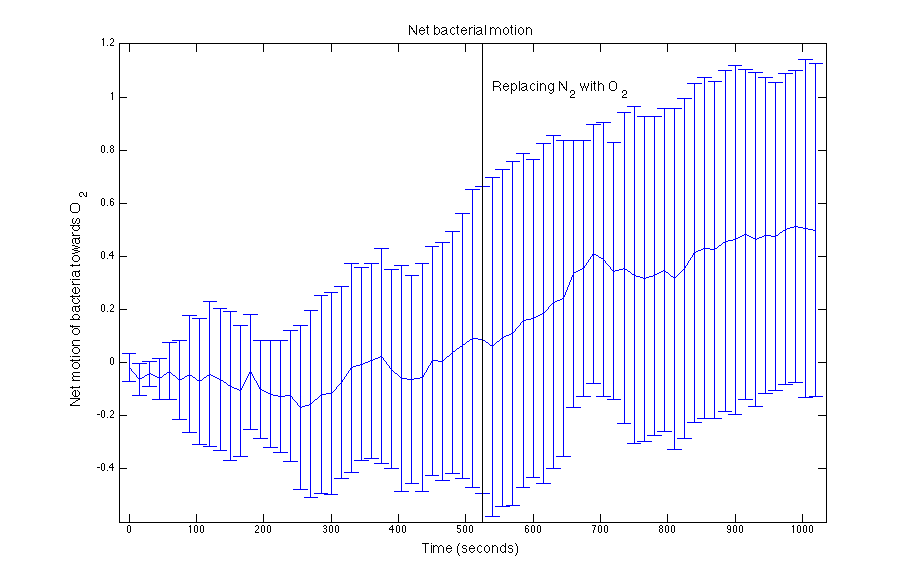
\includegraphics[width=\textwidth]{plots/cum_motion.png}
	\caption[Cumulative motion]{The cumulative percentage of net bacterial movement towards the oxygen side of the channel, averaged over 5 experimental trials. The x-axis is scaled relative to the number of visible bacteria in a single frame. \\
      
      This plot was produced by taking the cumulative sum of the difference between the ``left'' and ``right'' quadrants in the preceding figure. This sum is averaged over five trials. Error bars represent the standard deviation of that cumulative sum over the five trials (they grow with time because error is also being integrated in the cumulative sum). The size of the error bars is caused by a small $n$ (5), and integrated error. \\
      
      Note that there appears to be some drift prior to the gas line switch. This is likely due to random motion of the bacteria and the large uncertainty in the data.}
      
\end{figure}

\newpage
\newpage
\newpage
\newpage
\newpage
\newpage


\section{Discussion} % all of us
% figure refs need to be changed
% needs discussion of error sources

B. cereus failed to react noticeably to aerotaxis, so  we went back to a bacteria that had a documented response. We chose B. cereus initially because it was easier to culture and obtain.

B. subtilis did not react well to the initial fluorescent dye (SYTO 84 by Invitrogen), becoming non-motile and photobleaching quickly. Fluorescence imaging is much more effective for tracking the moving bacteria than brightfield, as bacteria can shift in and out of the focal plane easily. In brightfield, a bacteria shifting out of the focal plane will be lost by the tracking program, whereas in fluorescence, it has to shift a lot further from the focal plane to be lost.

The membrane dye (FM4-64) also didn�t produce useable data due to similar problems with the SYTO 84, so brightfield tracking was revisited.

The 10x objective was not sufficient for brightfield tracking, even though the depth of field was superior, so the 20x objective was utilized. Originally, images of each side of the channel were obtained over time to show the difference in bacterial concentration, but taking image data from the center of the channel will provide bacteria trajectories that are sufficient to discuss bacteria population movement.

With all the data processing performed, it was clear that qualitatively, B. subtilis does exhibit aerotactic behavior. In Figure 5, it can be noted that B. subtilis does tend to move towards the oxygenated side of the channel over time. Figure 6 also supports this behavior as it shows that bacteria density increases over time on the oxygenated side of the channel (the left of the graphs). Figure 7 displays counts of trackable bacteria on both the nitrogen side of the channel compared with the oxygen side of the channel, showing that over time, the majority of the bacteria migrate towards the oxygen. Figure 8 also shows that bacteria on the oxygenated side of the channel move at a faster average speed than those on the nitrogen side, which makes sense, as aerotaxis is an energy taxis and B. subtilis is also a facultative anaerobe, preferring aerobic respiration. Error sources for the qualitative analysis include 

However, attempts to utilize collected data to quantify the aerotactic response proved to be mostly futile. Basically, it was almost impossible to distinguish directed movement from random walks performed by the bacteria. In Figure 9, though there is noticeably more bacteria moving over time on the oxygen side, the directionality of both the oxygen and nitrogen sides are indistinguishable. The main reason for this lack of clarity is that brightfield tracking results in short bacteria tracks, as shown in Figure 12. These tracks are of varied lengths because bacteria would fall in and out of focus, either of which would disrupt the tracking program used to draw the tracks. There is no discernable difference or trend within each of the graphs as well. Figure 13 displays the motion of motile bacteria in 4 directions. Though there is more motion in the left/right directions than in up/down, there is still no significant difference between left and right in terms of overall trends. One would expect that aerotactic behavior would show an increase in leftwards (towards oxygen) motion over rightwards motion after the oxygen flow is turned on. However that is difficult to discern if at all in the graph.

There are many possible paths to continue these experiments. The first step would be to develop a working fluorescence method to more accurately track bacteria movements. This would improve the quality of data acquired and allow longer tracks to be monitored, helping to better distinguish between random walk motion and aerotactic behavior. The data acquired with brightfield displays very short tracks, meaning the bacteria fell out of the focal plane before the end of the experiment.

A second step to improve the experimental test bed would be to utilize a higher-quality microscope objective lens. This would improve the depth-of-field in the micrographs and also help with keeping bacteria relatively in focus, especially if fluorescence was utilized.

Finally, the microfluidic device could be made of a more inert material, such as glass. This would serve to keep the bacteria from sticking to the walls of the channel; however, glass is not gas-permeable, which is a necessity for aerotactic studies in microfluidics. 

\section{Conclusion}

While B. cereus does not respond to aerotaxis, B. subtilis demonstrates a weak but distinguishable response. Its aerotactic behavior was visually verified, as the bacteria tended to move towards the oxygenated side of the channel and away from the nitrogenated side, as seen in figure [graph containing population tracking trend]. The unsuccessful fluorescence system impeded efforts to quantify the aerotactic response of B. subtilis and produce a model analogous to those for chemotaxis, but figure [gradient] clearly demonstrates a qualitative response that further experiments could successfully quantify.

Our device provides a suitable testbed for conducting aerotaxis experiments, but it requires refinement to capture quantitative data. Some suggested improvements include a better fluorescence system using dye that does not impede bacterial movement or photobleach quickly, using a laser with a wavelength closer to the dye�s absorption peak. Improving the fluorescence system would improve the quality of tracking data, by allowing bacteria to be more reliably distinguished from the background, allowing additional insight into aerotactic behavior.

\section{Acknowledgements}

We�d like to thank Filippo Menolascina from the Center for Environmental Microfluidics for providing an introduction, masks, devices, supplies, and guidance throughout this project. We�d also like to thank Professor Nagle for assisting greatly with analysis of our data and the use of the 20.309 lab space, as well as ordering parts and supplies for us, and the 20.109 staff for allowing us to use their lab for bacteria culturing.


\begin{thebibliography}{9}

\bibitem{15years} Taylor, B.L, Igor B. Zhulin, and Mark S. Johnson. ``Aerotaxis and other energy-sensing behavior in bacteria.'' Annu Rev Microbiol. 1999;53:103-28.
\bibitem{modelI} Tindall, M.K., P.K. Maini, S.L. Porter, and J.P. Armitage. ``Overview of Mathematical Approaches Used to Model Bacterial Chemotaxis I: The Single Cell.'' Bull Math Biol. 2008 Aug;70(6):1525-69. doi: 10.1007/s11538-008-9321-6. Epub 2008 Jul 19.
\bibitem{modelII} Tindall, M.K., P.K. Maini, S.L. Porter, and J.P. Armitage. ``Overview of Mathematical Approaches Used to Model Bacterial Chemotaxis II: Bacterial Populations.'' Bull Math Biol. 2008 Aug;70(6):1570-607. doi: 10.1007/s11538-008-9322-5. Epub 2008 Jul 19.

\end{thebibliography}

\end{document}  